\subsubsection{Vorstellung des ``Pretzelboard''}        
\label{sec:Vorstellung des ``Pretzelboard''} 
Das ``Pretzelboard'' ist ein sogenanntes Elektronikmodul, dass unter verschiedenen Namen bekannt ist. Neben ``Pretzelboard'' ist der Name ``NanoESP-Board'' ebenfalls bekannt. Die Besonderheit des Boards ist ein bereits angeschlossenes \ac{WLAN} Modul, welches sowohl als Sender als auch Empfänger arbeiten kann. 

Da es zudem den gleichen Microcontroller wie das bekanntere Microcontrollerboard ``Arduino Uno'' nutzt, kann die Entwicklungsumgebung von Arduino zur Entwicklung von Software genutzt werden. 
Der Vorteil der bereits erfolgten Kombination und Verdrahtung von WLAN Modul und Microcontroller des Pretzelboards liegt darin, dass der Nutzer dies nicht mehr machen muss und somit wesentlich weniger Kenntnisse vorausgesetzt werden müssen (vgl. \cite{.b}\cite{.kafka}\cite{FranzisVerlagGmbH.27.11.2015}).

\begin{figure}[!htb]
	\centering
	\includegraphics[scale=0.4]{Pretzel.jpg}
	\caption[``Pretzelboard'']{``Pretzelboard'',\\ Quelle: http://cdn.pollin.de/article/xtrabig/X880281.2.JPG}
\end{figure}

\subsubsection{Verwendung im Projekt}        
\label{sec:Verwendung des ``Pretzelboard''} 
Das ``Pretzelboard'' wird im Projekt als Button genutzt. Sowohl die kleine Größe als auch die bereits vorhandene \ac{WLAN} Funktionalität sorgen dafür, dass sich das Board dafür besonders gut eignet. Aufgrund der Tatsache, dass es sich bezüglich der Programmierung nicht von einem Arduino Board unterscheidet, besteht die Möglichkeit, dass auf das Wissen und den Support einer bereits größeren Community zurückgegriffen werden kann. 

Da sich das Board zudem auf ein Elektroniksteckboard setzen lassen kann, ist auch die Verbindung mit einem Button und Statusleuchten möglich. Nach der erfolgreichen Montage kann dann das entsprechende Programm aufgespielt werden und bei vorhandener Stromversorgung kann die entsprechende Nachricht über das \ac{WLAN} Netzwerk an den Empfänger gesendet werden. Das Pretzelboard kommuniziert diese Nachricht mithilfe des zuvor bereits erwähnten Protokolls \ac{UDP} (vgl. Kapitel \ref{sec:UDP-1}).


\begin{figure}[!htb]
	\centering
	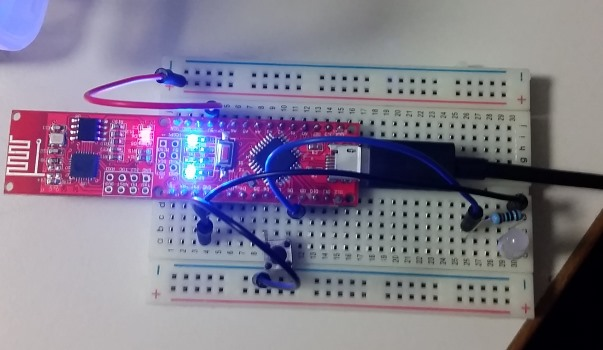
\includegraphics[scale=0.6]{Pretzel_Projekt.jpg}
	\caption[Pretzelboard im Projekt]{Pretzelboard im Projekt,\\ Quelle: Eigene Aufnahme}
\end{figure}
